\documentclass[10pt,a4paper]{article}
\usepackage[latin1]{inputenc}
\usepackage{amsmath}
\usepackage{amsfonts}
\usepackage{amssymb}
\usepackage{graphicx}
\title{Finite Element Method Computer Assignment 4.1.1}
\begin{document}

\begin{figure}[t]
	\centering
	
\includegraphics[width=0.5\textwidth]{TU_d_line_P1_color_1.jpg}
\end{figure}

\begin{center}
	\textbf{Computer Assignment 4.1.1}\\
	\textbf{MMP Finite Element Methods (WI4243AP-FE)}
\end{center}

\section{Introduction}
The following is a report containing the evaluation of the heat equation with the finite element method.
First the problem is defined followed by the derivation of the element matrix and vector.

\section{Problem formulation}
Consider a rectangular plate, with width, $b$, and height, $h$. In the center of the plate is a rectangular part, of a different material, with width, $b_0$ and height, $h_0$. $A$ denotes the outer part of the plate while $B$ denotes the inner part.

	\begin{figure}[t]
		\centering
		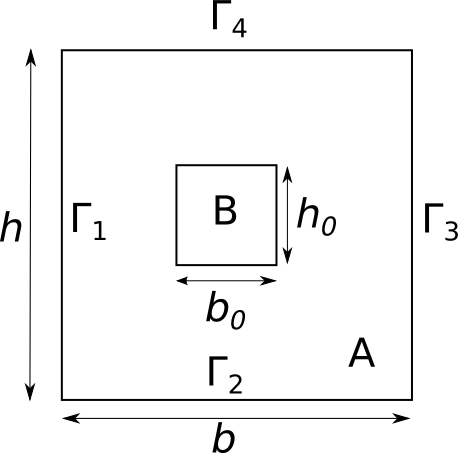
\includegraphics{schem.png}
		\caption{caption}
		\label{fig:schem}
	
	\end{figure}

Figure ~\ref{fig:schem} shows a schematic of the rectangular plate. The stationary heat equation is given by the two-dimensional equation 

\begin{equation}
	-\nabla \cdot (k \nabla T) = 0
\end{equation}

with heat conductivity $k$ and temperature $T$. The thermal conductivity is different in each material, i.e. $ k|_A = k_A $ and $k|_B = k_B $.

The boundary of $A$, $\partial A$,  is divided in four segments such that $\partial A = \Gamma_1 \cup  \Gamma_2 \cup  \Gamma_3 \cup  \Gamma_4$. On these boundaries the following conditions hold:

\begin{equation}
T|_{\Gamma_1} = T_0
\end{equation}

\begin{equation}
\nabla T|_{\Gamma_2} = T_0
\end{equation}

\begin{equation}
T|_{\Gamma_3} = T_0
\end{equation}

\begin{equation}
k\frac{\partial T}{\partial n}|_{\Gamma_4}=-\alpha(T_w - T_{\infty})
\end{equation}

In words, the temperature at boundaries $\Gamma_1$ and $\Gamma_3$ are held constant at $T=T_0$. The flux at $\Gamma_2$ is zero while $\Gamma_4$ obeys Newton's heat transfer relation with $T_{\infty}$ the environment temperature and $T_w$ the temperature at the wall.

\end{document}